\chapter{System Design and Verification}

\section{Introduction}

An outdoor pose measurement system is required. Due to their considerable cost, radar and laser measurement systems are not considered, which requires another method to be devised. One method that is investigated is using computer vision (CV) techniques to estimate the pose of a drone. 

The CV measurement system will make use of a flat calibration pattern and a Perspective n-Points (PnP) problem solver to extract the six-dimensional pose data vector $\bm{x} = {[x\;y\;z\;\theta\;\phi\;\psi]}^T$, where ${[x\;y\;z]}^T$ are the translation dimensions and ${[\theta\;\phi\;\psi]}^T$ are the roll, pitch and yaw dimensions respectively. 

This section discusses the details of the CV system implemented. It starts by discussing the system layout and design

\section{System Layout}

\subsection{Hardware}

The hardware requirements for the CV system are minimal. To perform six-dimensional pose estimation of a calibration pattern, either one or two cameras are required, along with a flat board containing the calibration pattern and a laptop running the pose estimation software. 

The accuracy between the single and stereo camera in most respects is rather negligible, except in the depth dimension, where the stereo vastly outperforms the single camera. This is to be expected and is very akin to a person's depth perception abilities being compromised with one eye closed. For this implementation, the single camera variant was selected. This makes the system simpler to set up and use. However, care must be taken with the depth estimation when using a single camera.

For the pose estimation software to work best, it requires a good view of the calibration pattern. Therefore, a big calibration pattern would be desirable. Furthermore, the pattern should of a high quality and printed on white paper with a wide white border to enhance the contrast between the pattern and the background, making it easier for the software to detect the pattern. 

\subsection{Software}
\label{sec:cv-sys-software}

The software used to perform the pose estimation comes packaged with the OpenCV computer vision library. 

The camera of the CV system is calibrated by a calibration function and pattern. The goal of the calibration process is to determine the intrinsic parameters of the camera matrix. The camera matrix takes up the form given in Equation~\ref{eq:cam-matrix},

\begin{equation}
  \label{eq:cam-matrix}
  P = 
  \begin{bmatrix}
    f_x & 0   & u_0 \\
    0   & f_y & v_0 \\
    0   & 0   & 1   \\
  \end{bmatrix}
  \begin{bmatrix}
    R | T
  \end{bmatrix}
\end{equation}

where $f_x$ and $f_y$ describe the focal lengths of the camera, and $u_0$ and $v_0$ are the principal points. $R$ is a $3\times3$ matrix describing the rotation of the camera, and $T$ is a three-dimensional vector describing the translation of the camera. 

To extract data from the image of a calibration board, a feature detection function from OpenCV is used. It scans the image and returns a set of two-dimensional data points of the features of the calibration pattern. Furthermore, a Random Sample Consensus (RANSAC) algorithm is used to discard any erroneous data points.

The transformation from two-dimensional image coordinates, $\bm{x}_c$, to to three-dimensional world coordinates, $\bm{x}_w$, is given by Equation~\ref{eq:2d-to-3d}.

\begin{equation}
   \label{eq:2d-to-3d}
   \begin{bmatrix}
     u & v & 1 \\
   \end{bmatrix}^T
   = P
   \begin{bmatrix}
     x_w & y_w & z_w & 1 \\
   \end{bmatrix}^T
 \end{equation}

With the camera matrix $P$ known, and a set of two-dimensional data points, a Principle n-Point (PnP) problem solving function can be used to extract the $R$ and $T$ matrices, describing the pose of the camera relative to the calibration board, from the data. The standard PnP solver, as described by~\cite{Schweighofer2006}, is used. The Efficient-PnP method, described by~\cite{Lepetit2008}, is more efficient, but requires more data points, which a typical calibration board may not have many of.

\section{Experiment Design}

Before the CV system can be used to record pose data of a drone, the accuracy of its measurements must first be determined. Since the PnP solving algorithm is, at its core, an optimisation problem and produces pose estimates, this is an important step in the system design phase. 

To determine the measurement error, a measurement test is performed in an indoor environment where an external measurement device records pose data. The error is then determined by comparing the CV system's data with that of the external measurement system's measurement data. Both systems were set to record the pose of a flat chessboard pattern that was moved and orientated by hand.

This section describes the experimental layout, including the external measurement device and its layout, as well as the CV system details. Then, the measurement procedure is presented, followed by the steps taken to process the data during the post-processing phase. Finally, the results of the experiment is given and discussed. 

\subsection{Experiment Layout}

\subsubsection{External Measurement Device Layout}

The external measurement system used to record the data that will be taken as ground-truth pose data, is a Vicon indoor motion capture system. It is a widely-used commercial system with applications in the film, medical and sporting industries and can reach millimetre accuracy in its measurements, depending on the individual set-up and how well its calibrated. It works by tracking a set of infrared markers stuck to a surface with at least two infrared cameras and sophisticated proprietary motion tracking software. Given its accuracy, the measurement results from this system is taken as ground-truth and the results from the CV system was compared to the Vicon system's to determine the CV system's measurement accuracy. 

The Vicon system used in this experiment is located in the 3D Human Motion Laboratory on Stellenbosch University's Tygerberg medical campus. It consists out of eight  infrared cameras arranged around a square on the floor in a configuration that maximises the number of markers visible to each camera at any given point in time. Figure~\ref{fig:vicon-layout} shows a diagram of the Vicon system layout. The Vicon cameras are set to capture at 300 FPS and some scaling was therefore required to match it to the 30 FPS that the CV system produces. 
 
\begin{figure}
  \centering
  \input{figures/chapter3/vicon_layout.pdf_tex}
  \caption{Layout of the Vicon system. Note that this is not drawn to scale.}
\label{fig:vicon-layout}
\end{figure}

Before the test commenced, the Vicon system was calibrated. For the experiment, markers were placed on both the calibration board and camera frame used by the CV system. Since the Vicon and CV camera each have their own coordinate systems, having the position and orientation of the CV camera available will allow the Vicon's measurements to be related back to the CV camera's coordinate system during the post-processing phase. 

The markers were placed in such a way that they will produce axes that more or less coincides with the Vicon's axis system, slightly reducing the work load during the post-processing phase. Figure~\ref{fig:cam-vicon-axes} shows the axis system's for both the CV and Vicon systems.

\begin{figure}
  \centering
  \def\svgwidth{0.6\textwidth}
  \input{figures/chapter3/cam_vicon_axis.pdf_tex}
  \caption{The axis orientations of the Vicon and CV systems.}
\label{fig:cam-vicon-axes}
\end{figure}

Only three markers are required for the Vicon system to produce a six-dimensional pose vector, but a fourth asymmetrical auxiliary marker was placed to provide fail-safe orientation data during the post-processing phase. Figures~\ref{fig:cam-marker-placement} and~\ref{fig:board-marker-placement} show the marker placements for the camera and calibration board. These markers were carefully placed by hand, but they will have some error associated with them, which is to say there is an offset between the marker placement and the point that will be estimated by the Vicon system. This offset is taken into account during the post-processing phase.

\begin{figure}
   \centering 
   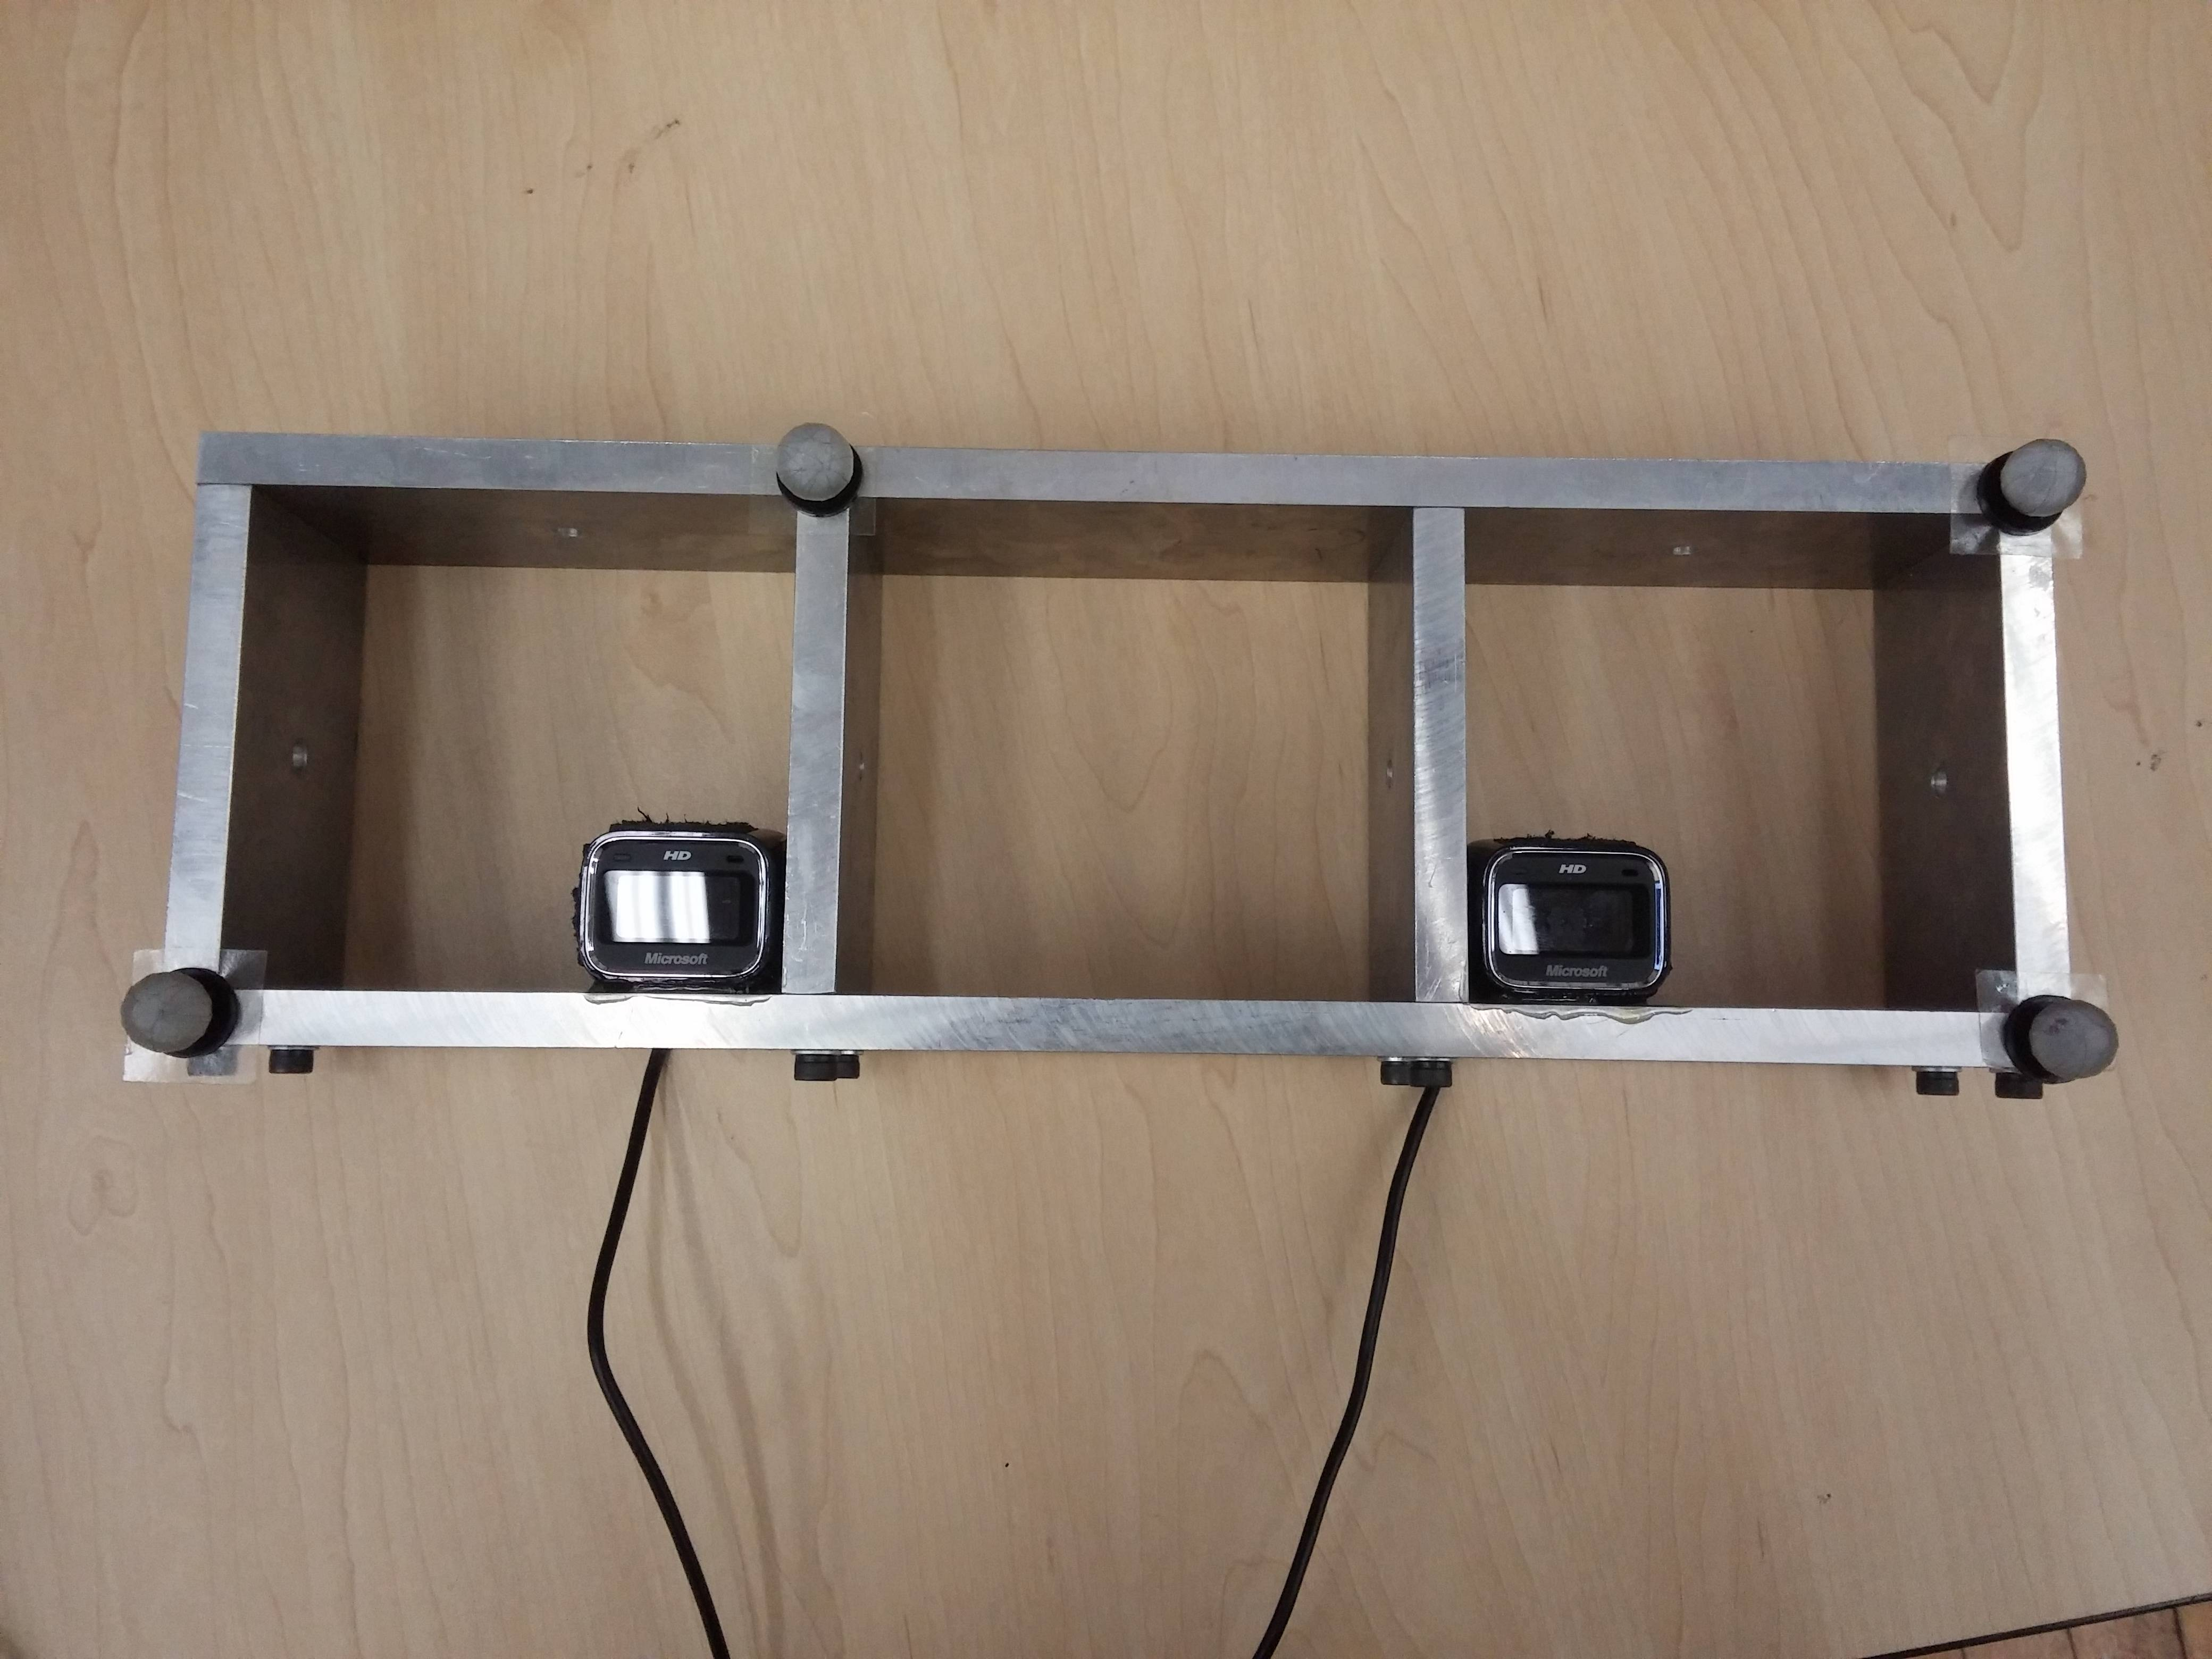
\includegraphics[width=0.8\textwidth]{figures/chapter3/cam_1_low}
   \caption{Infrared marker placement on the camera.}
\label{fig:cam-marker-placement}
\end{figure}

\begin{figure}
   \centering 
   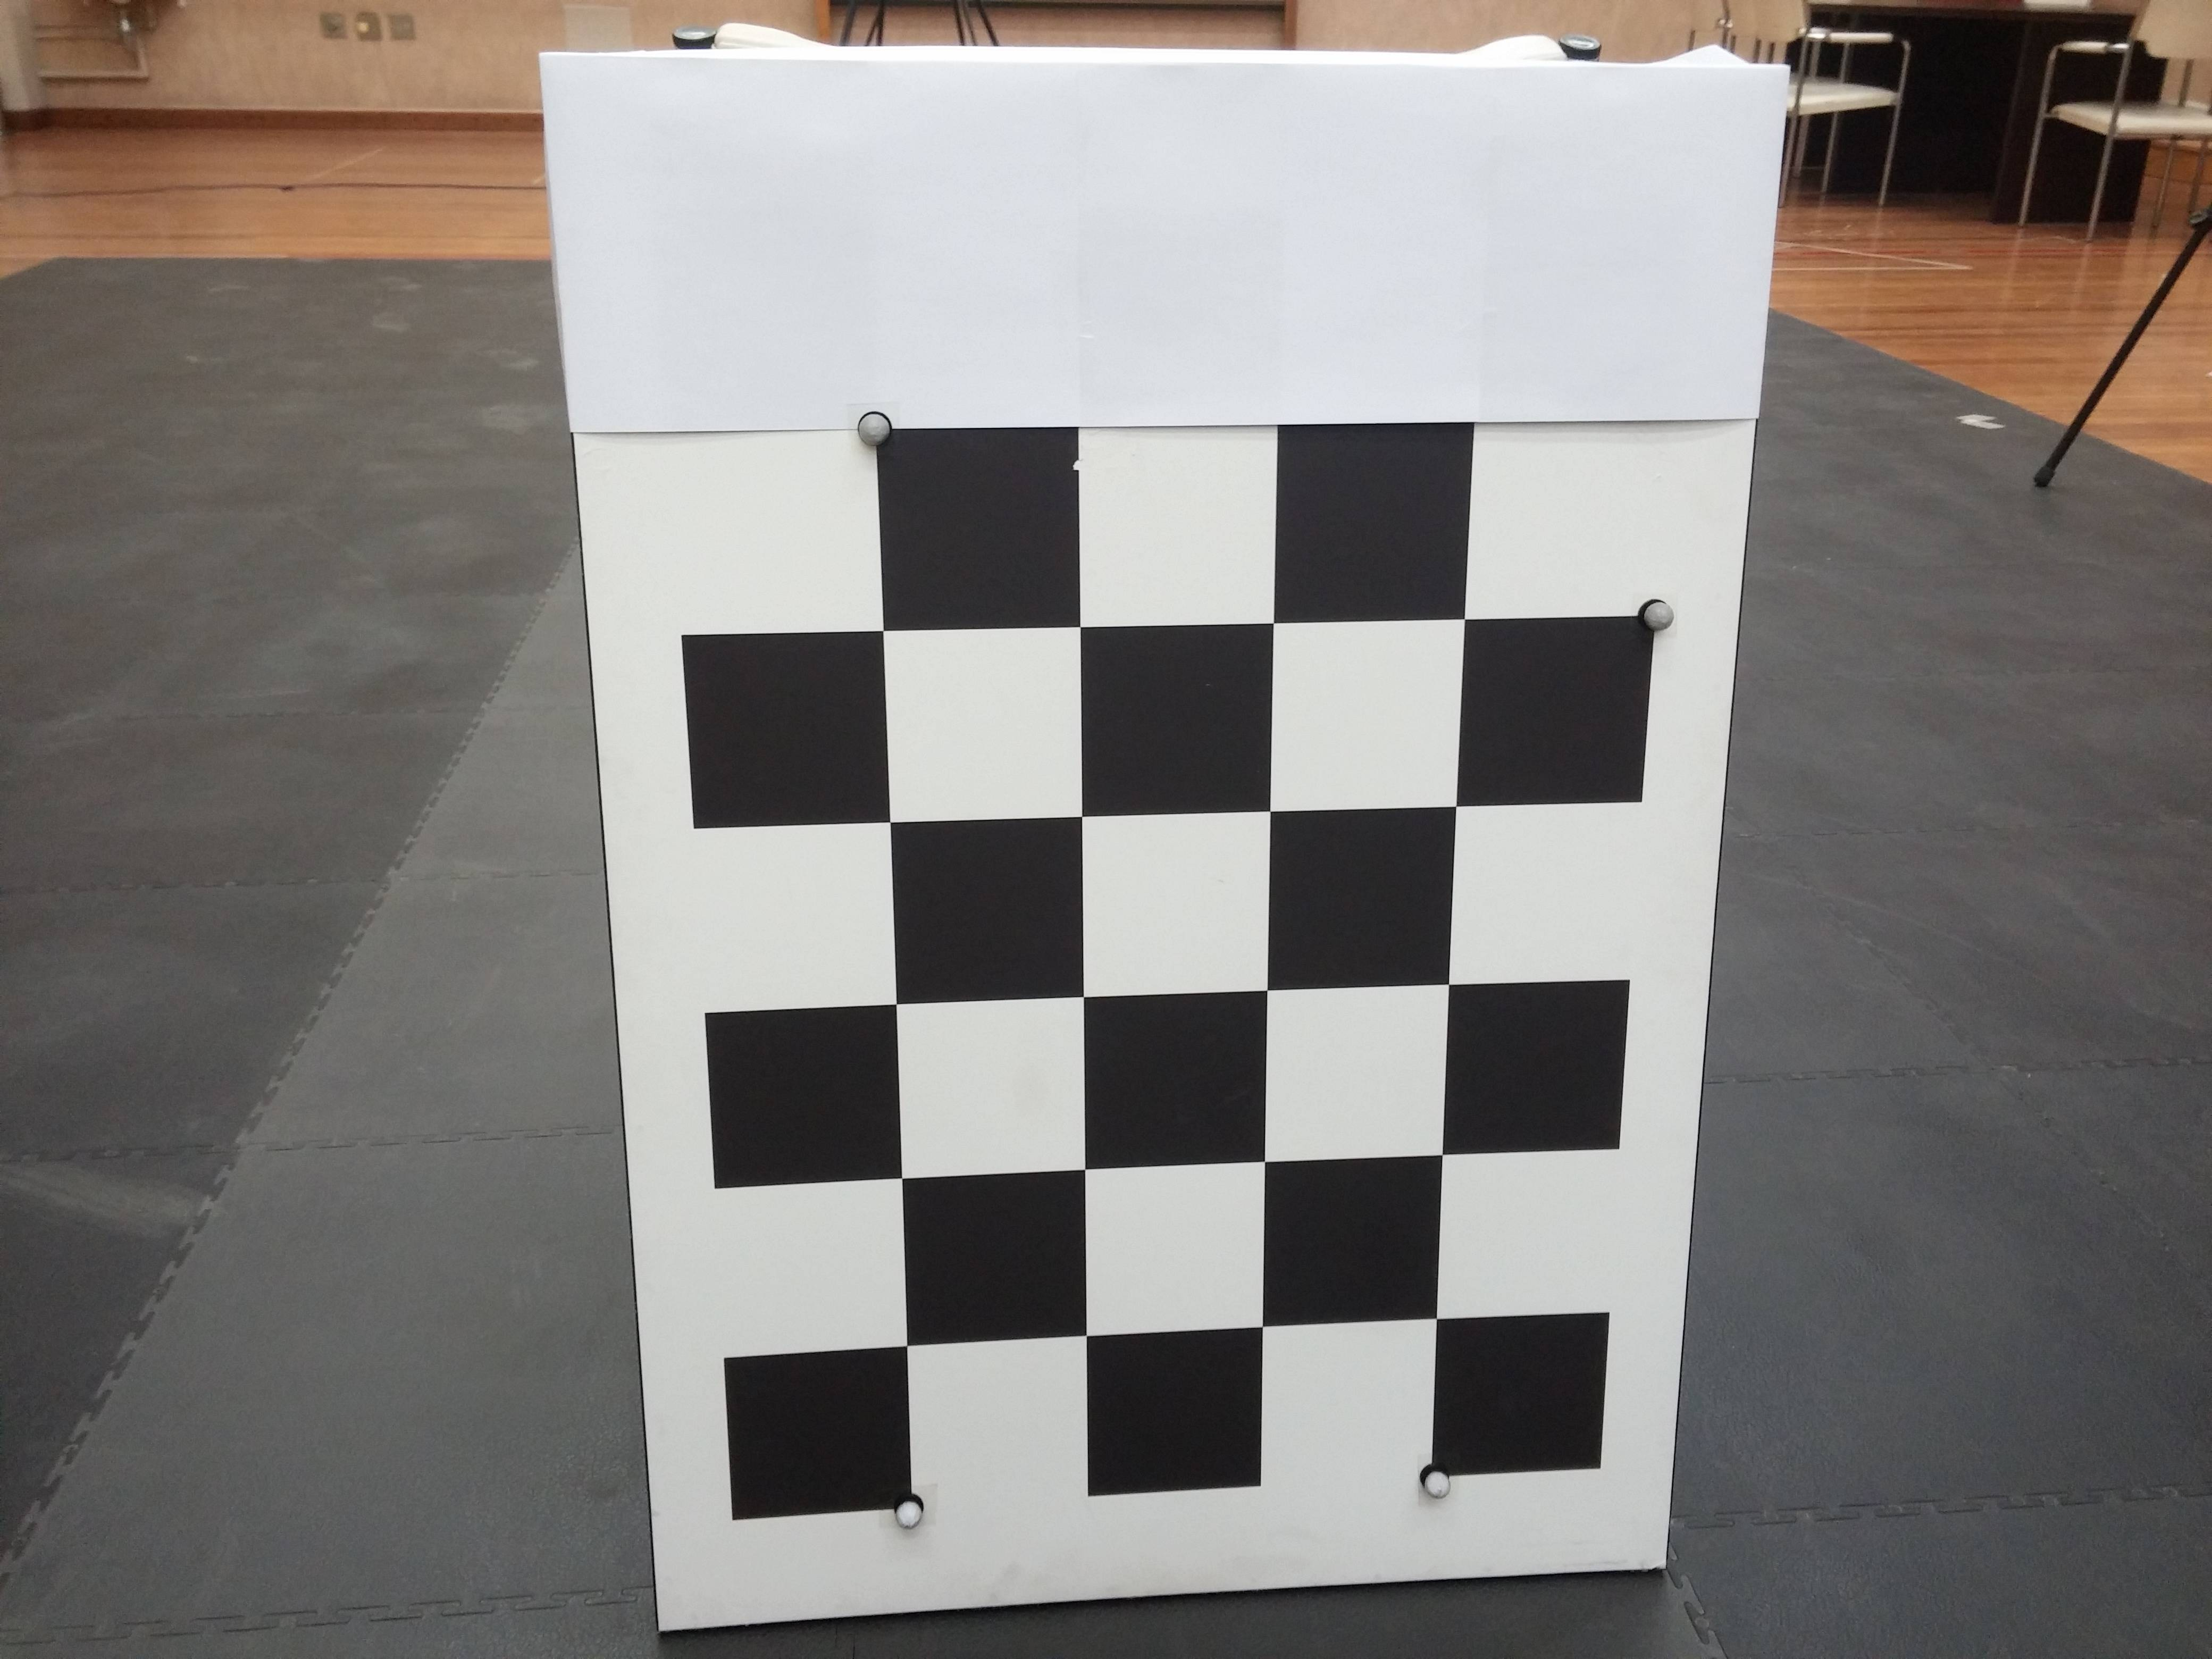
\includegraphics[width=0.8\textwidth]{figures/chapter3/bord_2_low}
   \caption{Infrared marker placement on the chessboard.}
\label{fig:board-marker-placement}
\end{figure}

One aspect of the Vicon system to note is that the infrared markers have some high-frequency noise associated with them, which is apparent when inspecting the raw data. This noise is inherent to the marker and can be safely filtered out with a zero-lag Butterworth filter. However, the raw, unfiltered data is used throughout this project. 

\subsubsection{CV System Setup}

\subsection{Experiment Procedure}

\subsection{Data Processing}

\section{Results}

\section{Conclusion}

